\chapter{Analisi del problema}


In questo capitolo si fornisce una descrizione del problema.

%
% Commento: questa � la prima sezione
%
\section{Titolo sezione}

\index{Titolo per indice della sezione}

Qui inseriamo un riferimento \cite{a}.

\subsection{Titolo sottosezione}

\begin{figure}[tp]
    {\begin{center}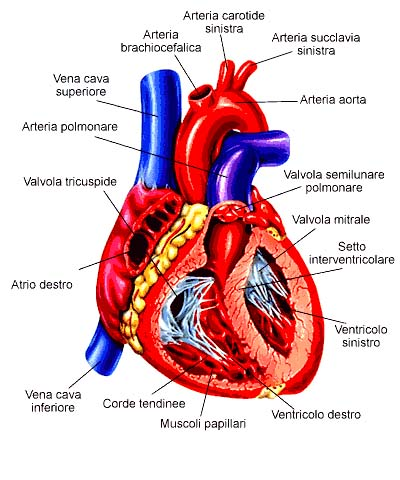
\includegraphics[width=8cm]{figure/cuore_aperto.jpg}\end{center}}
\caption{Il cuore  \label{cuore}}
\end{figure}

Come si vede in figura \ref{cuore}...

Riferimento ad un sito \cite{mysite}...

\subsection{Seconda sottosezione}

bla bla